\subsection{A lower AI weight and a higher efficiency bound}
\label{subsec:rewrite-low-ai-price-calibration}

Table~\ref{tab:rewrite-low-ai-price-parameters} lists the full configuration,
including the changed upper bound and the recalibrated research productivity.
\begin{rewriteParameterTable}{Lower AI weight: parameters and initial stocks}{tab:rewrite-low-ai-price-parameters}
$\omega_X$ & 0.10 & AI production weight & Arbitrary lower-weight scenario, not fitted to the industry's size; zero before date zero.\\
$\omega_L$ & 0.90 & Effective-labor weight & $1-\omega_X$; one before date zero.\\
$\chi$ & 36.031845 & Research productivity & Refitted at $\sigma=1$ to $p_X(2.25)/p_X(0)=0.20$; same approximate OECD target \citep{oecdaimarkets2026}.\\
$\sigma$ & 0.90; 1; 1.10; 1.50 & AI--labor substitution & Arbitrary scenarios; the fitted $\chi$ is shared across all four.\\
$\overline B$ & 1,360.992139 & AI-efficiency upper bound & $1.10\mathcal B(1.50)$ evaluated at $\omega_X=0.10$; arbitrary 10\% margin chosen to keep $\sigma=1.50$ AI-dominated.\\
\midrule
$A_0,N_0$ & 1; 1 & Initial technology and population & Unit normalizations.\\
$K_0$ & 5.941573 & Initial capital & Calculated no-AI Ramsey steady state, Equation~\eqref{eq:rewrite-ramsey-start-stocks}.\\
$B_0$ & 13.609921 & Initial AI efficiency & $0.01\overline B$; arbitrary initial distance from the higher bound, not an estimate.\\
\end{rewriteParameterTable}

I repeat the price-calibrated comparison with $\omega_X=0.10$ and
$\omega_L=0.90$, starting AI efficiency at $1\%$ of its upper bound.
Reducing the AI weight raises the threshold for AI domination. At
$\sigma=1.50$, halving $\omega_X$ multiplies $\mathcal B(1.50)$ by eight,
from approximately $154.66$ to $1{,}237.27$. To keep this case in the
AI-dominated regime, I retain the previous margin above the threshold:
\begin{equation}
 \overline B=1.10\,\mathcal B(1.50)=1{,}360.9921,\qquad
 B_0=0.01\overline B=13.6099.
 \label{eq:rewrite-low-ai-price-stocks}
\end{equation}
These numbers are rounded; the simulations use the exact threshold formula.
The upper bound is eight times the preceding value. Although $B_0/\overline B$
falls from $10\%$ to $1\%$, the level of $B_0$ falls by only $20\%$, from
$17.0124$ to $13.6099$.

I again set $A_0=N_0=1$ and use the no-AI Ramsey capital stock
$K_0=5.9416$ from \eqref{eq:rewrite-ramsey-start-stocks}.
The economy begins with this inherited capital stock because the experiment
introduces AI into an economy previously on the no-AI steady state.
The initial AI-efficiency ratio remains illustrative. I retain $\eta=0.20$
and all macroeconomic parameters, and solve initial consumption and the
developer's shadow value anew. I recalibrate $\chi$ at $\sigma=1$ to the
same approximate OECD price target in \eqref{eq:rewrite-price-calibration-target},
then hold it fixed across the four elasticities. Here the target implies
$B(2.25)=0.05\overline B$, rather than $0.50\overline B$ in the preceding
comparison. The same observed price decline therefore leaves much more room
for subsequent efficiency gains relative to the assumed upper bound.

The fitted value is $\chi\simeq36.03$, compared with $51.76$ in the
preceding experiment. This difference is not an estimate of a change in
research productivity: the two fits use different AI weights, initial
efficiency levels, and upper bounds. Both inherit the same limitations of
the quality-adjusted API price index as a proxy for $p_X$. The final
unit-elastic path still matches the price target after both horizon
extensions. Over the same 27 months, prices fall by $31.8\%$, $84.5\%$,
and $91.2\%$ at $\sigma=0.90,1.10,$ and $1.50$, respectively; these are
model predictions conditional on the common $\chi$, not additional targets.

Figures~\ref{fig:rewrite-low-ai-price-accumulation}--
\ref{fig:rewrite-low-ai-price-distribution} retain the same panels,
normalizations, and two time windows as the preceding comparison.
All four paths pass the same equilibrium-admission tests, including the
dense checks over the initial ten years.

\begin{figure}[H]
 \centering
 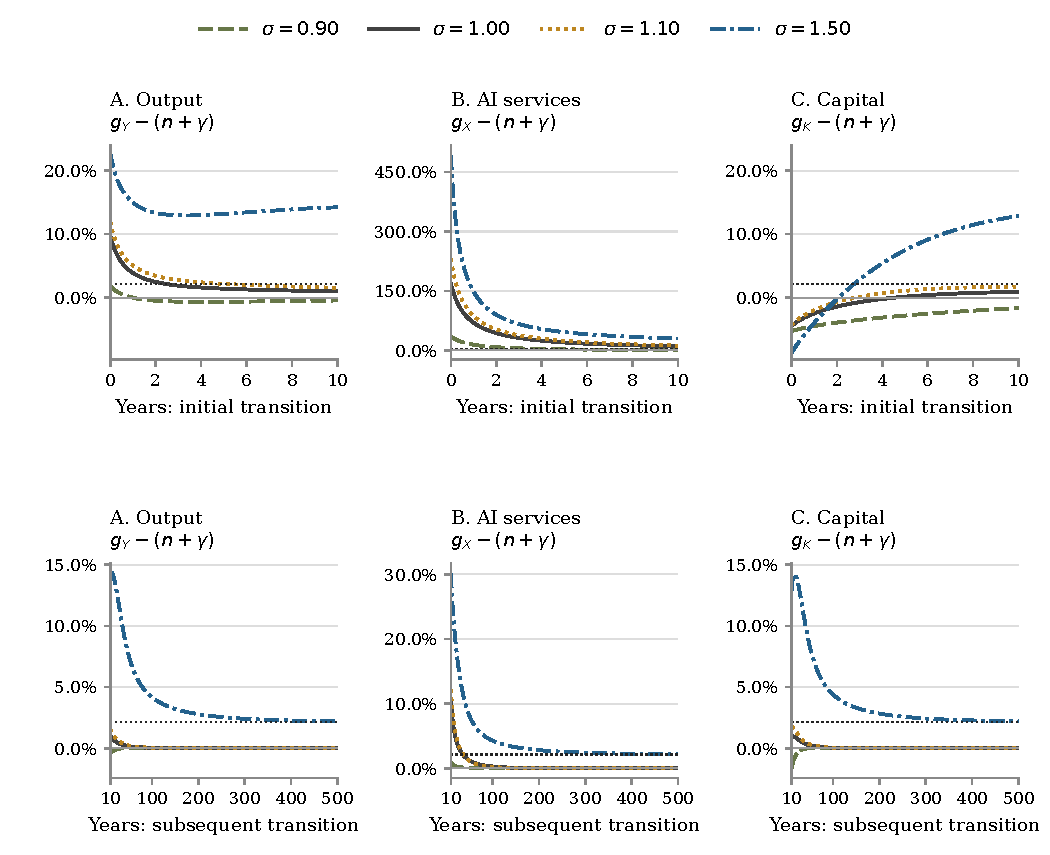
\includegraphics[width=\textwidth]{figures_rewrite/equilibrium_price_calibrated_low_ai_high_cap_accumulation_growth_windows.pdf}
 \caption{Lower-weight price calibration: growth of output, AI production
 services, and capital per unit of effective labor. The upper row shows
 years 0--10; the lower row shows years 10--500, with separate vertical
 ranges. Rates are instantaneous annual rates, not realized one-year
 changes. Panels A and C share a vertical scale within each row.
 Dotted lines mark the analytical limits for $\sigma=1.50$.}
 \label{fig:rewrite-low-ai-price-accumulation}
\end{figure}

Initial output-per-person growth ranges from $2.8\%$ at $\sigma=0.90$ to
$23.8\%$ at $\sigma=1.50$, compared with $21.6\%$ and $113.2\%$ in the
preceding experiment. These are instantaneous annual rates. At
$\sigma=1.50$, real wages initially grow at $11.0\%$, rather than $54.4\%$.
The smaller initial expansion does not produce a prolonged interval near
the $1\%$ labor-bottleneck benchmark: output-per-person growth remains
$14.2\%$ after 27 months and $15.2\%$ after ten years.

\begin{figure}[H]
 \centering
 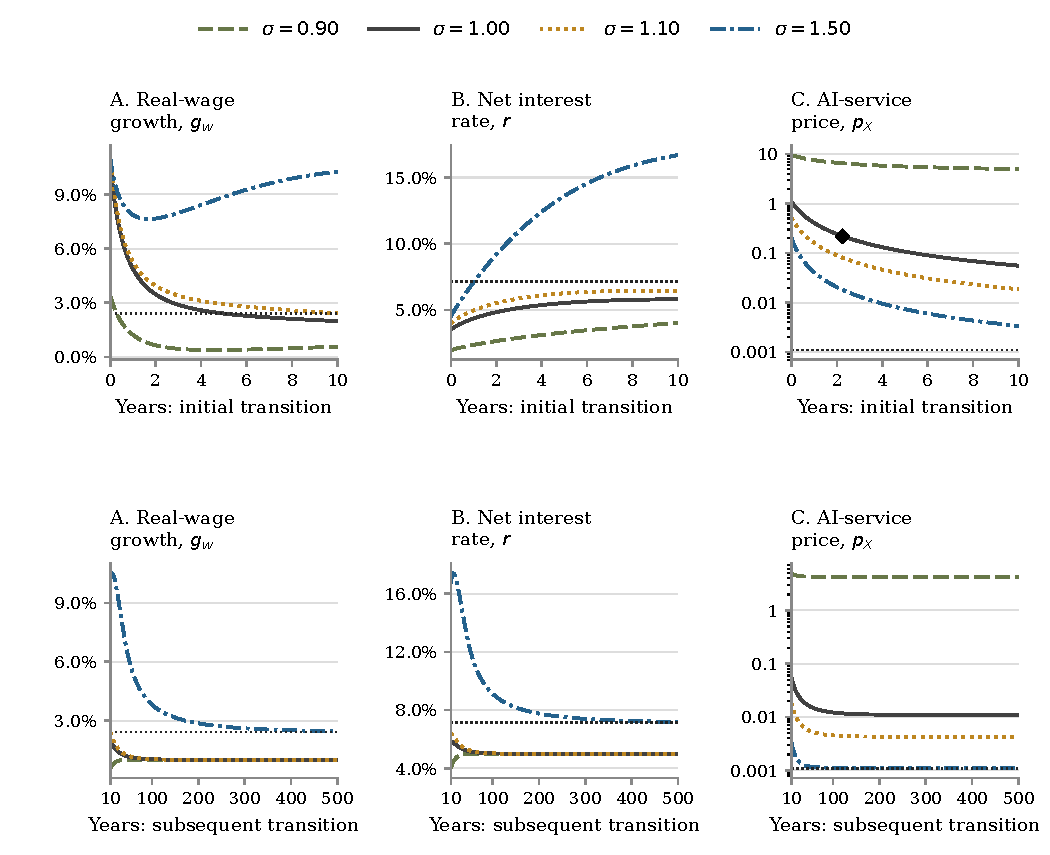
\includegraphics[width=\textwidth]{figures_rewrite/equilibrium_price_calibrated_low_ai_high_cap_growth_returns_windows.pdf}
 \caption{Lower-weight price calibration: real-wage growth, the net
 interest rate, and the AI-service price. The upper row shows years 0--10;
 the lower row shows years 10--500. Rates use linear percentage scales
 and $p_X$ uses a logarithmic scale. The black diamond marks the same
 27-month price target, scaled to this experiment's initial unit-elastic
 price; it is not an observed absolute price in model units.
 Dotted lines mark the analytical limits for $\sigma=1.50$.}
 \label{fig:rewrite-low-ai-price-returns}
\end{figure}

At $\sigma=1.50$, labor initially receives $61.8\%$ of output, falling to
$51.2\%$ after 27 months and $33.9\%$ after ten years. Half of its decline
toward zero takes $11.9$ years, versus $3.0$ in the preceding comparison;
$90\%$ takes $60.5$ years, versus $51.7$. The net interest rate begins at
$4.52\%$, below the $5\%$ labor-bottleneck benchmark, and rises to
$9.66\%$ after 27 months. Rapid efficiency improvement and the distributional
transition need not occur at the same speed.

\begin{figure}[H]
 \centering
 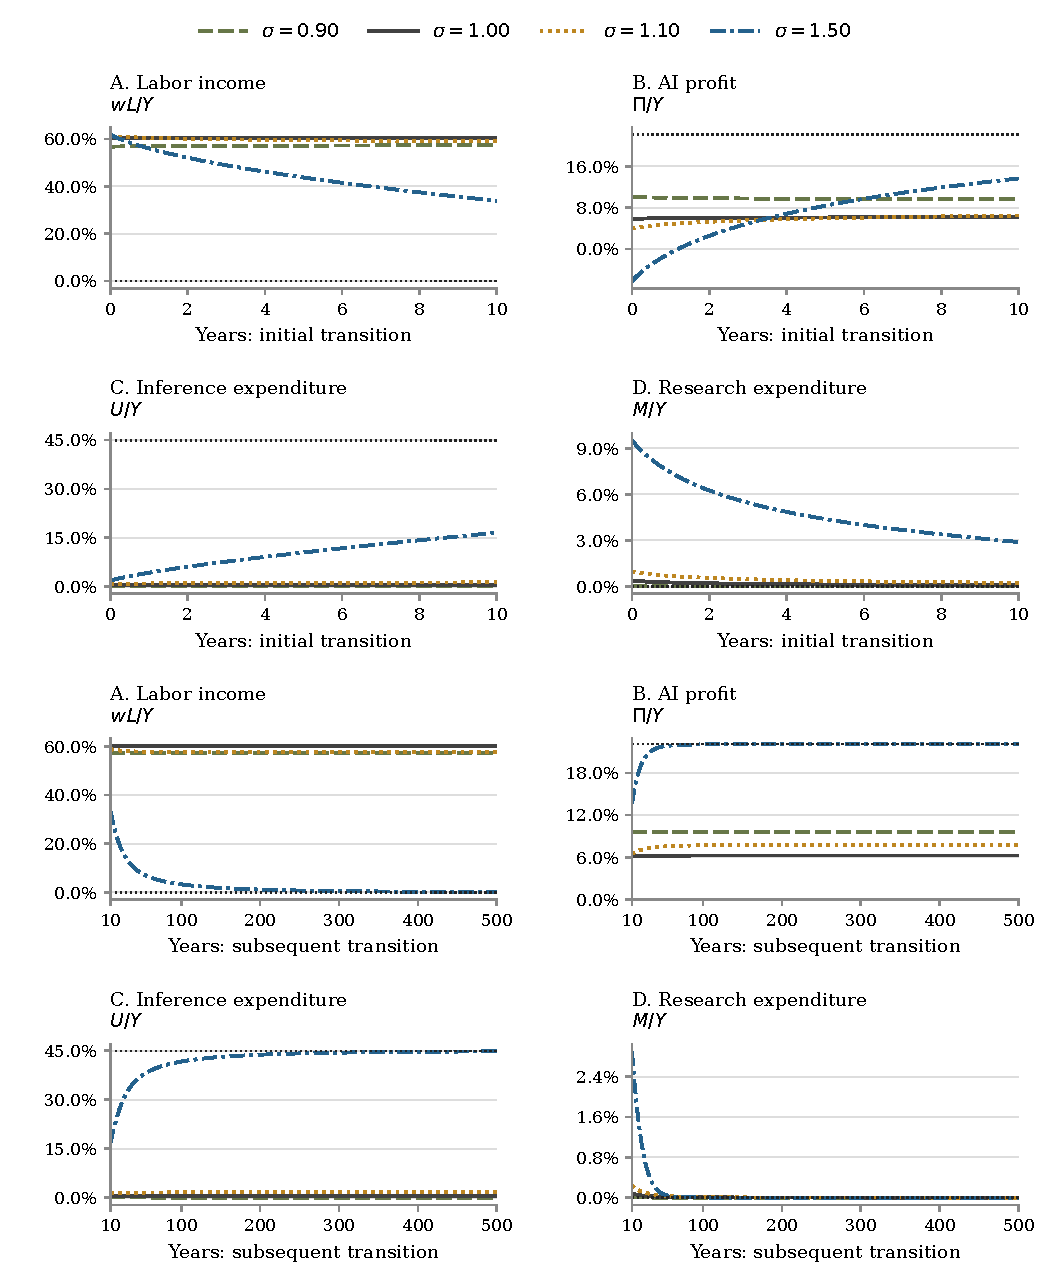
\includegraphics[width=\textwidth,height=0.83\textheight,keepaspectratio]{figures_rewrite/equilibrium_price_calibrated_low_ai_high_cap_ai_distribution_windows.pdf}
 \caption{Lower-weight price calibration: labor income, AI net profit,
 inference expenditure, and research expenditure as shares of output.
 The first two rows show years 0--10; the last two show years 10--500,
 with separate vertical ranges. The shares sum to $1-\alpha$; gross
 capital income remains $\alpha$. Negative profit denotes financing by
 the household owner. Dotted lines mark the analytical limits for
 $\sigma=1.50$.}
 \label{fig:rewrite-low-ai-price-distribution}
\end{figure}

\begin{samepage}
The lower AI weight does not eliminate the initial financing requirement.
At $\sigma=1.50$, AI revenue initially represents $5.2\%$ of output,
compared with $17.0\%$ previously. Research expenditure falls from
$13.7\%$ to $9.5\%$ of output, but net profit falls from $-3.9\%$ to
$-6.2\%$: the decline in revenue exceeds the decline in inference and
research expenditure. Research absorbs
$182.6\%$ of AI revenue, and net profit is $-118.5\%$ of that revenue.
The household owner finances this temporary loss against future monopoly
profits. Capital per unit of effective labor initially contracts in all
four cases, before rising in the $\sigma=1.50$ economy.

\end{samepage}

The three labor-bottleneck cases still approach $1\%$ output-per-person
and real-wage growth and a $5\%$ net interest rate. At $\sigma=1.50$,
the long-run rates remain $3.135\%$, $2.423\%$, and $7.135\%$,
respectively, with labor's share approaching zero. These rates are
unchanged because the increase in $\overline B$ exactly offsets the lower
AI weight in the expression for $R(\overline B)$ at this elasticity.
The comparison changes the transition and the terminal levels in the
labor-bottleneck cases, not the terminal growth-rate contrast.

This is a joint sensitivity exercise: the AI weight, the initial efficiency
ratio, the upper bound, and the fitted $\chi$ all change. It does not isolate
the effect of any one parameter. Initial AI revenue ranges from $5.2\%$ to
$10.2\%$ of output across the four cases; at unit elasticity it is always
$6.7\%$. These shares have not been matched to the current AI industry.
The experiment remains a price-calibrated equilibrium comparison, not a
forecast of aggregate growth.
